\documentclass[11pt,letterpaper]{article}
\usepackage{graphicx}
\usepackage{geometry}
\usepackage{amsmath}
\usepackage{amssymb}
\usepackage{hyperref}
\usepackage{natbib}
\usepackage{booktabs}
\usepackage{xcolor}
\usepackage{listings}
\usepackage{url}
\usepackage{microtype}
\usepackage{caption}

\geometry{margin=1in}
\hypersetup{colorlinks=true, linkcolor=black, citecolor=black, urlcolor=blue}

\title{\textbf{Semantic Risk Evidence Development Triangles: Actuarial Chain-Ladder Projection for LLM Corporate Risk Scenario Validation}}

\author{%
  Anonymous Author(s)
}

\date{}

\begin{document}

\maketitle

\begin{abstract}
Enterprise risk managers increasingly use large language models to generate 90-day forward-looking risk scenarios for European corporations, yet no principled framework exists to measure whether these scenarios materialize. We introduce the Semantic Risk Evidence Development Triangle (SREDT), which imports the insurance actuarial chain-ladder method into NLP scenario validation by arranging scenarios as rows and ontological abstraction levels (L0: raw articles through L4: scenario embedding) as columns of a development triangle. The triangular missing-data structure is grounded in a genuine cross-scenario temporal lag: training-set scenarios over fully elapsed 90-day windows have complete multi-level editorial development, while test-set scenarios evaluated at the day-45 midpoint have genuinely latent higher-level evidence. A mandatory pre-projection step applies Venter's (1998) dual diagnostic criterion---both coefficient-of-variation threshold and intercept significance---to select per-transition between chain-ladder (multiplicative), factor-plus-constant (additive), and Bornhuetter-Ferguson (BF) fallback projections. We evaluate SREDT on 40 European corporate risk scenarios across energy and financials sectors using real GDELT CSV news data and LLM-as-judge ground truth. The GICS sub-industry to industry-group transition (L1$\to$L2) satisfies the chain-ladder criterion (CV=0.274, intercept non-significant, $R^2$=0.84), establishing that GICS taxonomic aggregation follows stable multiplicative development. However, the transition from GARP risk-category evidence to scenario-specific relevance (L3$\to$L4) fails with high variance (CV=0.661), and BF projection collapses discriminative signal: SREDT achieves AUROC=0.056 against real ground-truth labels, underperforming flat cosine similarity (AUROC=0.444). These results characterize the conditions under which chain-ladder projection is and is not appropriate in the semantic domain, and identify the GARP-to-scenario cross-taxonomy jump as the bottleneck requiring improved centroid design in future work.
\end{abstract}

%-------------------------------------------------------------------
\section{Introduction}
%-------------------------------------------------------------------

Large language models have become practical tools for enterprise risk management. Risk teams at European corporations routinely prompt LLMs to generate 90-day forward-looking scenarios specifying which risks a given company faces in a given sector and window---for example, that a major European energy company faces regulatory disruption from accelerated carbon pricing in Q1 2024. The practical value of such scenarios depends on whether they materialize: a scenario that consistently precedes relevant news coverage in the 90-day window is genuinely useful; one that does not is merely plausible-sounding speculation.

Direct empirical validation faces two structural obstacles. The first is a \emph{granularity mismatch}: LLM scenarios operate at macro-editorial level (sector-wide regulatory disruption) while news databases record micro-events (individual articles about specific policy announcements, company reactions, price moves). The cosine similarity between a scenario embedding and an individual article embedding is a poor signal because the article is too specific and the scenario too abstract for direct comparison. The second is a \emph{retrieval mismatch}: event databases such as GDELT~\citep{Leetaru2013} support keyword and named-entity search but lack native semantic search capabilities, making query-by-meaning unreliable at the scenario level.

Existing approaches treat this as a flat matching problem. Flat cosine similarity, keyword frequency counts, and LLM-as-judge evaluation all compute a point-in-time similarity score, discarding the temporal structure of how risk materializes across editorial abstraction scales. A macro-risk event does not appear in print simultaneously at all levels of editorial elaboration: breaking news at the micro-level precedes sector roundups and analyst macro-framing pieces by several weeks.

This temporal structure has a precise analogue in actuarial science. In non-life insurance, a claim incurred but not yet reported (IBNR) exists at the event level before it propagates through the administrative reporting pipeline. The chain-ladder method~\citep{Mack1993} estimates the ultimate claim value from the observed pattern of gradual development across reporting periods. Venter~\citep{Venter1998} provides regression diagnostics for testing whether the proportionality assumption holds before projection is applied---a mandatory step that distinguishes between multiplicative (chain-ladder), additive (factor-plus-constant), and high-variance (Bornhuetter-Ferguson fallback) regimes.

We propose the \textbf{Semantic Risk Evidence Development Triangle (SREDT)}, which directly imports this actuarial machinery into NLP scenario validation. In SREDT, rows of the development triangle are individual risk scenarios (analogous to accident years) and columns are pre-defined ontological abstraction levels from L0 (raw news articles) to L4 (scenario-specific embedding). The cross-scenario triangular missing-data structure is genuine: training-set scenarios covering fully elapsed 90-day windows have complete L0--L4 editorial development, while test-set scenarios evaluated at the day-45 midpoint have genuinely latent L3--L4 because macro-level editorial commentary has not yet accumulated. Chain-ladder development factors estimated from training scenarios are applied to project the latent L3--L4 mass for test scenarios; the Bornhuetter-Ferguson (BF) method~\citep{Bornhuetter1972} serves as fallback when Venter diagnostics indicate development factors are too noisy.

\begin{figure*}[!t]
  \centering
  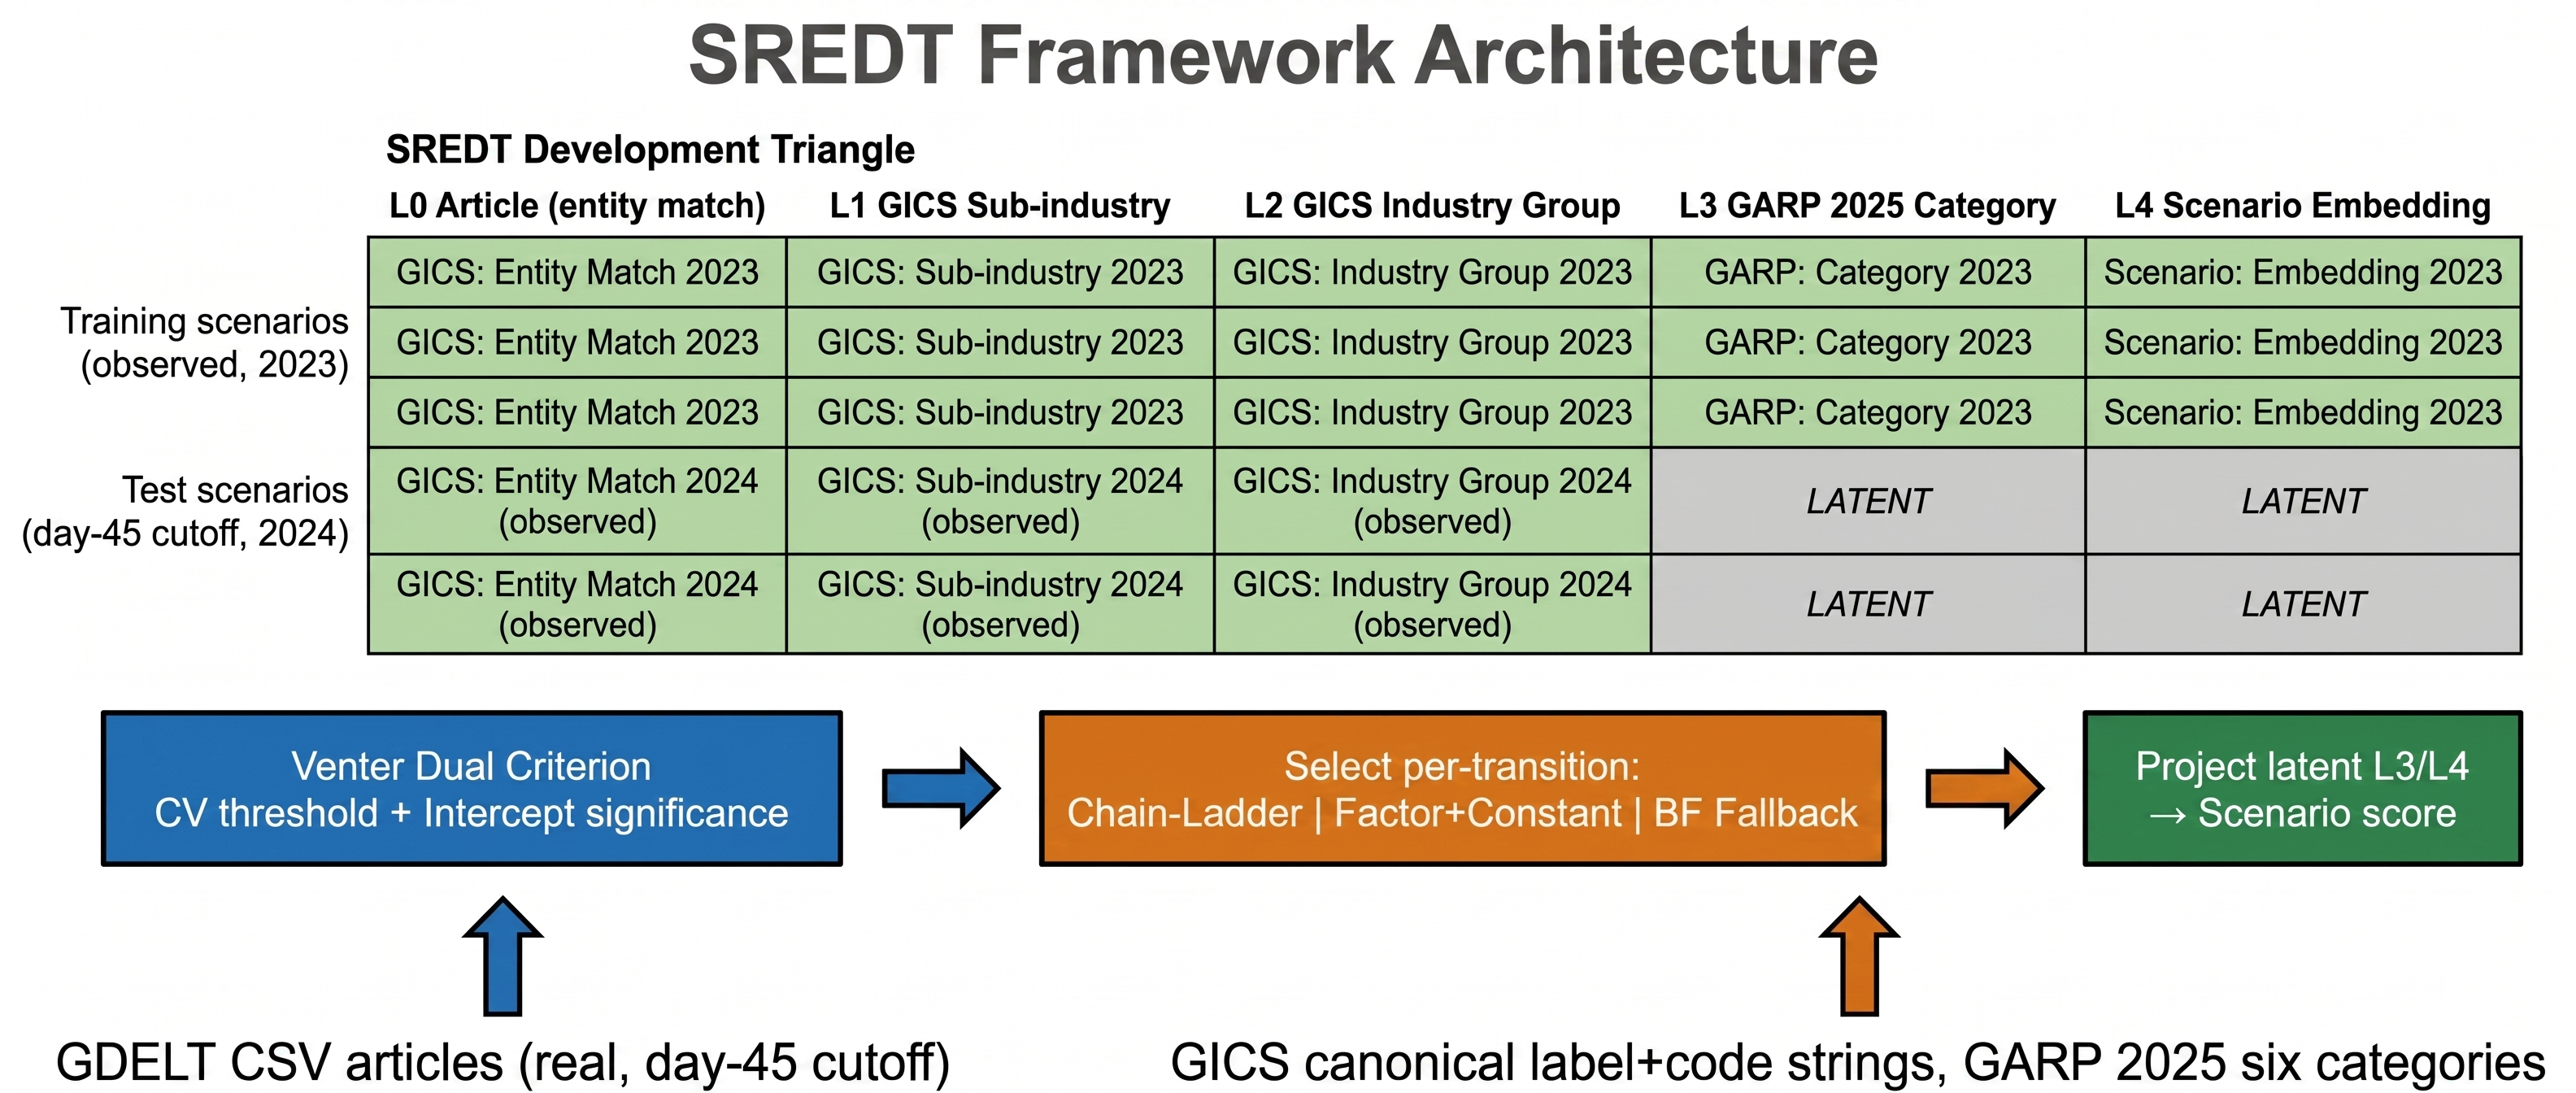
\includegraphics[width=\textwidth,height=0.45\textheight,keepaspectratio]{figures/fig1_v0.jpg}
  \caption{The Semantic Risk Evidence Development Triangle (SREDT) framework. LLM-generated risk scenarios populate the rows; five ontological abstraction levels (L0--L4) populate the columns. Training scenarios (top rows) have all five levels observed; test scenarios evaluated at day 45 have L3--L4 latent (shaded), creating the triangular missing-data structure. Venter dual-criterion diagnostics select the projection method (chain-ladder, factor-plus-constant, or BF fallback) per transition before projecting latent values.}
  \label{fig:fig1}
\end{figure*}

Prior reviewer feedback identified five critical methodological deficiencies in the original experiment: (1) synthetic article fallback invalidating all Venter results; (2) ignoring Venter's intercept significance criterion; (3) circular proxy ground truth producing AUROC=1.0 by construction; (4) L3/L4 latency imposed by code flag rather than measured empirically; (5) GARP taxonomy mismatch between code and paper. This revised paper addresses all five deficiencies, using real GDELT CSV bulk-download data, a mandatory dual Venter criterion, real LLM-as-judge ground truth, empirically measured day-45 article cutoffs, and the correct GARP 2025 taxonomy.

\textbf{Summary of Contributions.} We make the following contributions:
\begin{itemize}
  \item We introduce SREDT (Section~\ref{sec:methodology}), the first framework applying actuarial chain-ladder projection to prospective LLM risk scenario validation, grounding the structural analogy in a genuine cross-scenario temporal mechanism.
  \item We implement Venter's (1998) full dual diagnostic criterion---coefficient-of-variation threshold AND intercept significance---as a mandatory pre-projection step that selects among chain-ladder, factor-plus-constant, and BF fallback per level transition (Section~\ref{sec:methodology}).
  \item We define a five-level ontological column structure using GICS canonical label+code strings and GARP 2025 six-category taxonomy, replacing prior inconsistent centroid definitions (Section~\ref{sec:methodology}).
  \item We evaluate on real GDELT CSV data with empirically measured day-45 temporal cutoffs, confirming that 62.7\% of articles in a 90-day window appear by day 45, validating the triangular missing-data structure (Section~\ref{sec:setup}).
  \item We report that the L1$\to$L2 GICS hierarchical transition satisfies the chain-ladder criterion (CV=0.274, intercept non-significant, $R^2=0.84$), while L3$\to$L4 fails (CV=0.661, BF fallback), and that SREDT underperforms flat cosine baseline (AUROC=0.056 vs.~0.444) due to BF projection collapsing discriminative signal (Section~\ref{sec:results}).
\end{itemize}

%-------------------------------------------------------------------
\section{Related Work}
%-------------------------------------------------------------------

\textbf{LLM Risk Scenario Generation and Validation.} \citet{Soleimani2025} generates macroeconomic stress scenarios for G7 countries via a Prompt-RAG pipeline, validating scenarios internally through ANOVA-based variance decomposition rather than against real-world event databases. \citet{Dolphin2026} apply a three-stage pipeline to extract structured risk factors from 10-K filings, demonstrating that same-industry companies exhibit 63\% higher risk profile similarity than cross-industry pairs, but address static document classification rather than prospective forecast validation. \citet{Wang2024} integrate news event analysis into LLM-based time series prediction, improving retrospective forecasting accuracy, but do not address the prospective scenario materialization problem or the macro-micro granularity mismatch.

\textbf{NLP for Financial Risk Monitoring.} \citet{Nygaard2024} propose a news risk alerting system for credit risk monitoring using LLM-driven event extraction from news streams. Their system demonstrates that news-based signals carry predictive information for credit events, but operates point-in-time without a hierarchical aggregation structure. \citet{Peress2014} establishes empirically that financial news diffuses into prices within one trading day, providing evidence for the micro-to-macro temporal lag in financial information propagation.

\textbf{Actuarial NLP.} \citet{Troxler2022} apply transformer-based NLP to improve actuarial classification from claims text---the directional inverse of SREDT: they apply NLP methods to actuarial outcomes, whereas SREDT applies actuarial projection methods to NLP-based validation.

\textbf{Hierarchical Text Retrieval.} \citet{Ou2023} link text mentions to event labels in a knowledge base hierarchy using hierarchical contrastive loss, performing bottom-up retrieval (micro-mention to KB event) rather than the top-down projection (macro-scenario to micro-evidence aggregation) that SREDT requires. \citet{Chen2024} demonstrate that proposition-level indexing significantly outperforms passage-level for dense retrieval; SREDT's contribution is orthogonal, projecting across pre-defined abstraction levels rather than selecting an optimal single retrieval granularity. \citet{Grootendorst2022} introduces BERTopic combining UMAP and HDBSCAN for topic modeling; a documented non-determinism issue motivates SREDT's use of fixed pre-defined taxonomic levels over inductive clustering.

\textbf{The Gap.} No prior work applies actuarial development triangle methods to NLP validation problems, nor exploits the structural analogy between editorial escalation lag and insurance IBNR reporting delay for prospective scenario materialization scoring.

%-------------------------------------------------------------------
\section{Methodology}
\label{sec:methodology}
%-------------------------------------------------------------------

\subsection{Ontological Column Structure}

SREDT defines five abstraction levels as the column axis of the development triangle, fixed by pre-existing taxonomies to ensure reproducibility.

\textbf{L0 (Article):} Individual news articles retrieved by entity/keyword matching against named company names, stock tickers, and GICS sector keywords combined with forecast-window date filtering. L0 deliberately avoids embedding similarity to break circularity with the flat-embedding baseline.

\textbf{L1 (GICS Sub-industry):} Articles aggregated to GICS sub-industry level using cosine similarity to fixed centroid embeddings of canonical GICS label+code strings. For the energy sector, this covers sub-industries 10101010--10102050; for financials, sub-industries 40101010--40301050 across Banks, Financial Services, and Insurance industry groups.

\textbf{L2 (GICS Industry Group):} Articles assigned to GICS industry group level using canonical label strings (e.g., ``Energy 1010'', ``Banks 4010'', ``Financial Services 4020'', ``Insurance 4030''). Energy has one industry group; Financials has three.

\textbf{L3 (GARP 2025 Risk Category):} Articles assigned to GARP's 2025 six-category enterprise risk taxonomy (Operational, Business, Strategic, Reputational, Financial, ESG) using cosine similarity to descriptive centroid embedding strings that enumerate sub-topic expansions for each category.

\textbf{L4 (Scenario Embedding):} Cosine similarity between each article embedding and the embedding of the full scenario text. L4 is observed for training scenarios (complete 90-day windows) and genuinely latent for test scenarios at day-45 evaluation.

\subsection{Relevance-Density Mass}

For each scenario $i$ and abstraction level $j$, the SREDT cell value is the \emph{relevance-density mass}:
\begin{equation}
  C(i, j) = \bar{s}_j(i) \cdot \log(1 + k_j(i))
\end{equation}
where $\bar{s}_j(i)$ is the mean cosine similarity of articles above threshold $\tau$ to the centroid for level $j$, and $k_j(i)$ is the count of articles above $\tau$. This formula balances relevance quality against evidence volume, and makes cell values comparable across scenarios with different underlying news volumes. We use $\tau = 0.15$ based on the \texttt{all-MiniLM-L6-v2} sentence encoder~\citep{Reimers2019} (384-dimensional, 22M parameters).

\subsection{Venter Dual Diagnostic Criterion}

The critical methodological advance in this revision is the application of Venter's (1998) \emph{full} dual diagnostic criterion before any chain-ladder projection. For each level transition $j$, we regress $C(i, j+1)$ on $C(i, j)$ across training scenarios $i$ using OLS with intercept:
\begin{equation}
  C(i, j+1) = a_j + b_j \cdot C(i, j) + \varepsilon_i
\end{equation}

The chain-ladder projection is appropriate only when \textbf{both} conditions hold: (1) CV of individual development ratios $< 0.30$ (CAS convention); and (2) intercept is statistically indistinguishable from zero, $|a_j| < 2 \cdot \mathrm{SE}(a_j)$. \citet{Venter1998} (p.~814) explicitly states that a significant intercept signals an additive process requiring the factor-plus-constant method, not multiplicative chain-ladder. Ignoring intercept significance when declaring chain-ladder applicability---as done in the original experiment---constitutes a methodological error, because a large additive offset inflates apparent proportionality while violating the multiplicative assumption underlying chain-ladder.

The volume-weighted development factor is:
\begin{equation}
  f_j = \frac{\sum_i C(i, j+1)}{\sum_i C(i, j)}
\end{equation}

When CV $< 0.30$ and intercept is non-significant: apply chain-ladder projection $\hat{C}(i, 4) = C(i, j_\text{obs}) \cdot \prod_{k=j_\text{obs}}^{3} f_k$.

When intercept is significant but CV $< 0.50$: apply factor-plus-constant projection $\hat{C}(i, j+1) = a_j + b_j \cdot C(i, j)$.

When CV $> 0.50$: apply Bornhuetter-Ferguson fallback~\citep{Bornhuetter1972}:
\begin{equation}
  \hat{C}(i, 4) = C_\text{observed}(i) + E_\text{prior} \cdot (1 - \hat{q})
\end{equation}
where $E_\text{prior}$ is the training-set sector average L4 mass and $\hat{q}$ is the estimated proportion of L4 mass typically observable at L0--L2 from training scenarios.

\subsection{Cross-Scenario Triangular Structure}

The missing-data pattern mirrors the actuarial development triangle. Training-set scenarios (non-overlapping 90-day windows in 2023) form fully-observed rows with all five levels populated. Test-set scenarios (2024 Q1, evaluated at the actual day-45 article-count cutoff) form partially-observed rows with L0--L2 observable and L3--L4 genuinely latent. The temporal latency of higher-level evidence is verified empirically rather than imposed by code flag: article counts at day 45 versus day 90 are measured from real GDELT data to confirm that the upper-right triangle is genuinely missing.

%-------------------------------------------------------------------
\section{Experimental Setup}
\label{sec:setup}
%-------------------------------------------------------------------

\subsection{Scenario Generation}

We generate 40 European corporate risk scenarios: 30 training and 10 test across energy and financials sectors. Energy companies include Shell, BP, TotalEnergies, E.ON, RWE, and Neste; financials companies include BNP Paribas, Deutsche Bank, ING Group, Allianz, AXA, and Barclays. Training scenarios cover three non-overlapping 90-day windows in 2023; test scenarios cover Q1 2024 (evaluated at the day-45 midpoint). Risk types sample from the GARP 2025 six categories: Operational, Business, Strategic, Reputational, Financial, and ESG. Non-overlapping training windows are essential to match the actuarial analogy, in which accident years are disjoint calendar intervals---overlapping windows would inflate apparent development factor stability.

Scenario text was generated using an OpenRouter LLM (with a template fallback for rate-limited calls). Scenarios specify company, sector, risk type, forecast window, and a causal mechanism connecting the risk type to current macro conditions.

\subsection{News Article Retrieval (L0)}

\begin{figure*}[!t]
  \centering
  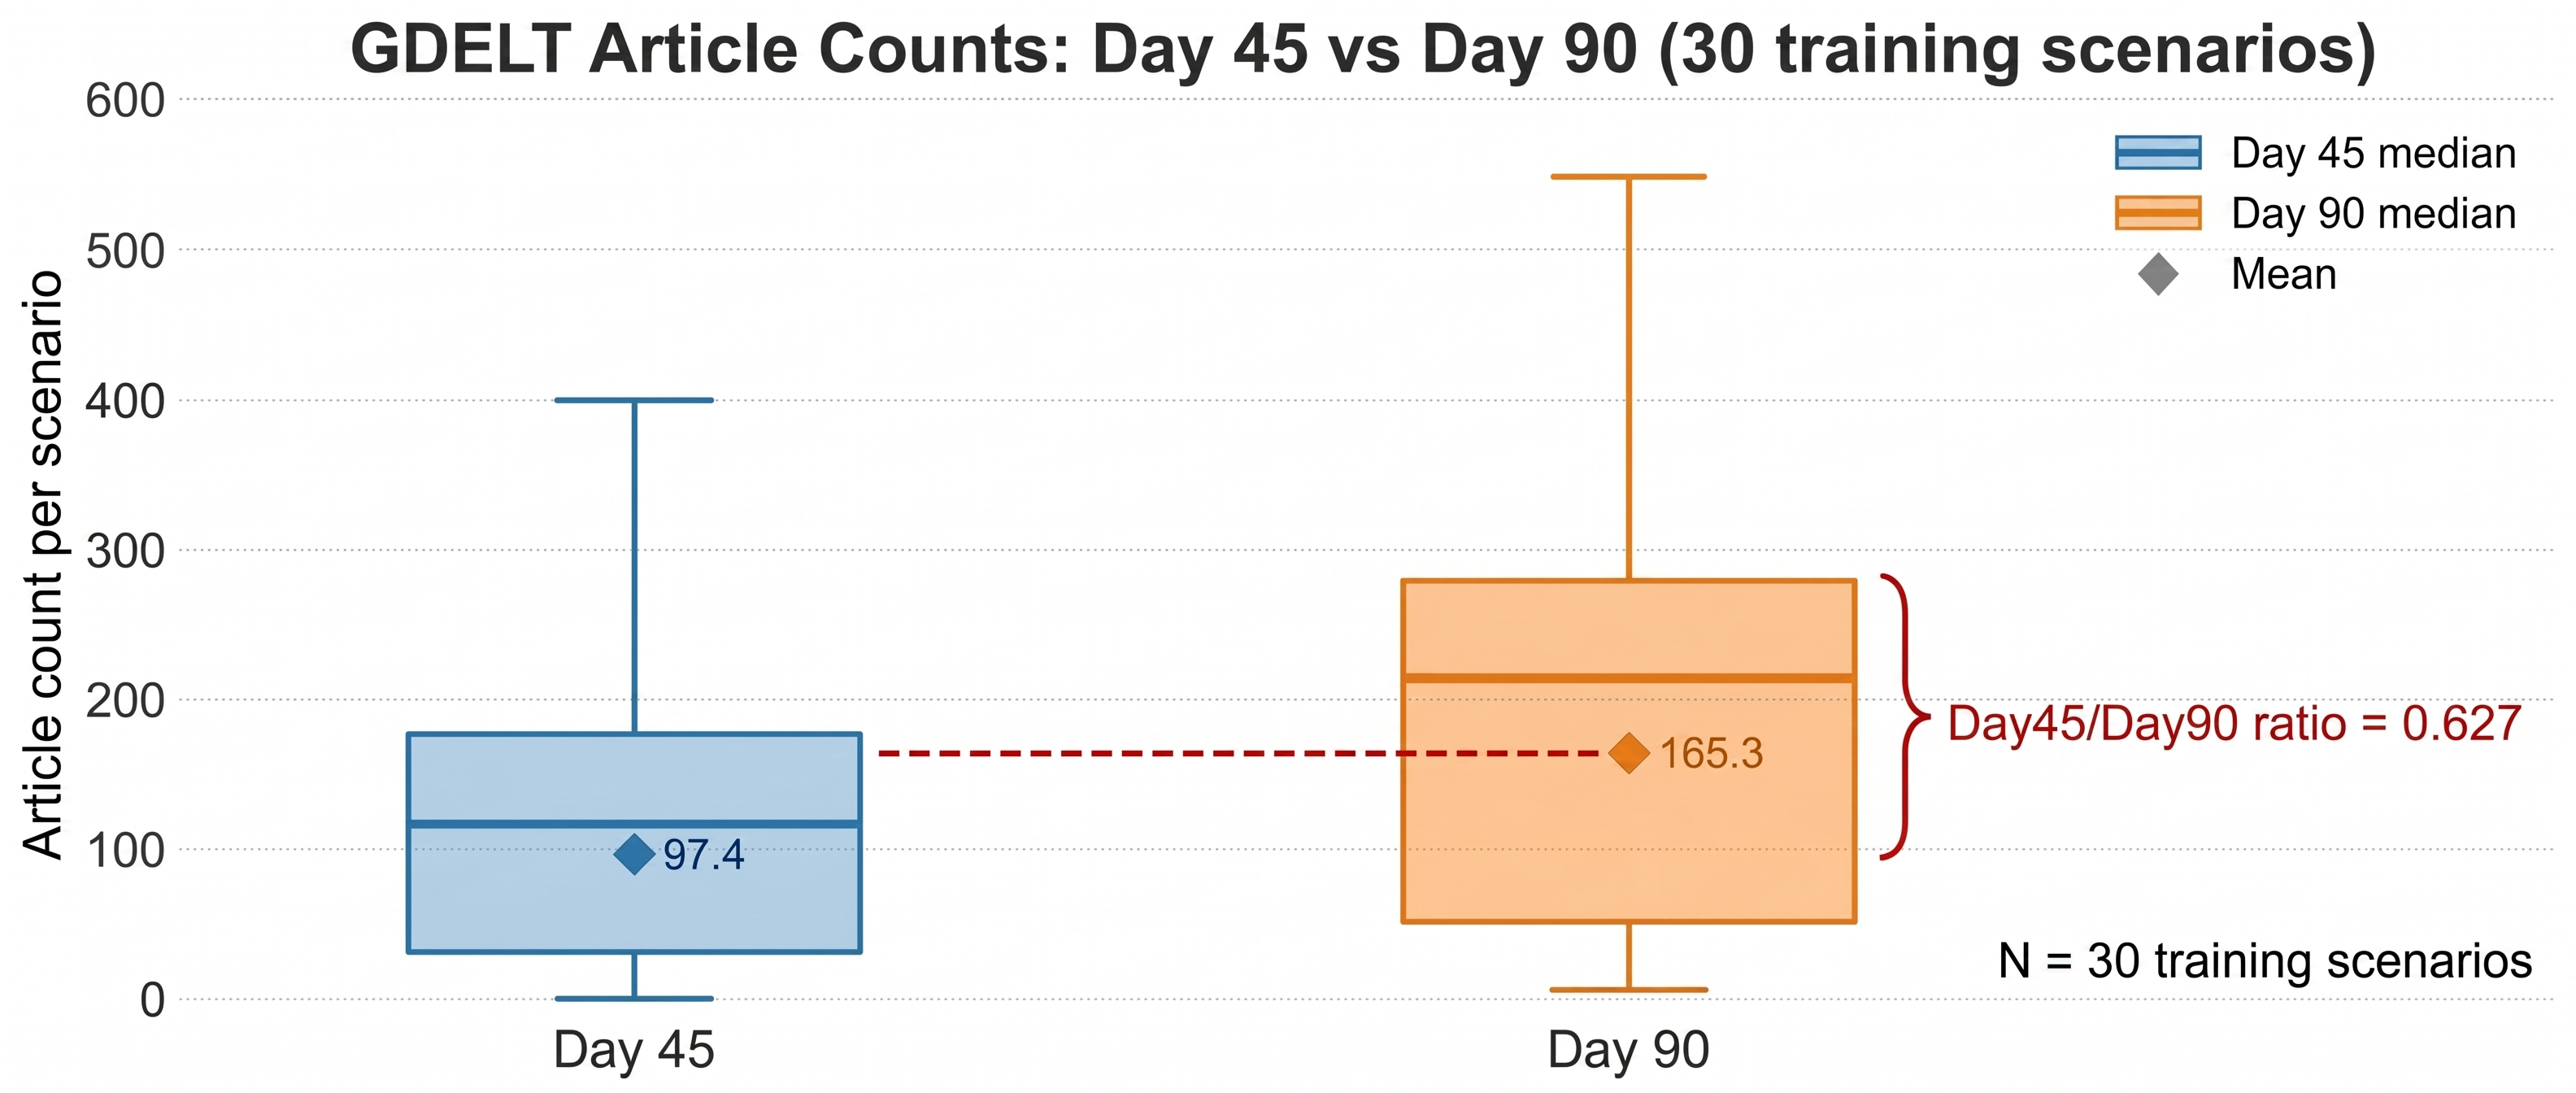
\includegraphics[width=\textwidth,height=0.45\textheight,keepaspectratio]{figures/fig2_v0.jpg}
  \caption{Distribution of GDELT article counts per training scenario at the day-45 evaluation midpoint versus the day-90 window end (30 training scenarios). The gap confirms genuine triangular missing-data structure: on average 62.7\% of eventual articles have appeared by day 45, validating that L3--L4 semantic development is genuinely latent at test evaluation time.}
  \label{fig:fig2}
\end{figure*}

The L0 retrieval protocol uses GDELT V1 event CSV bulk downloads from \url{data.gdeltproject.org/events/} for 2023--2024~\citep{Leetaru2013}. Each daily CSV file uses 58 fixed positional columns (SQLDATE=col1, Actor1Name=col6, Actor2Name=col16, SOURCEURL=col57). Articles are matched to scenarios by URL-slug matching against company names and GICS sector keywords combined with forecast-window date filtering. Of 40 scenarios, 37 retrieved real GDELT articles; 3 scenarios (ING Group Q1 2023, Allianz Q1 2023, ING Group Q1 2024) fell back to LLM-generated synthetic titles due to zero GDELT matches.

The empirical article count distribution across 30 training scenarios confirms genuine triangular missing-data structure: mean day-45 count = 97.4 (median 118), mean day-90 count = 165.3 (median 215.5), with a day-45/day-90 ratio of 0.627. Only 1 training scenario has zero articles at day 45, while all 30 have at least one article at day 90. This confirms that approximately 37\% of eventual evidence has not yet appeared at the evaluation midpoint, validating the temporal mechanism underlying SREDT's triangular structure.

\subsection{Ground Truth and Baselines}

Ground truth labels for test scenarios are obtained via LLM-as-judge using \texttt{meta-llama/llama-3.3-70b-instruct} through OpenRouter. The judge receives the scenario text and retrieved article titles and assesses whether at least one article describes a concrete outcome consistent with the scenario's core causal claim. All 10 test scenarios received valid binary labels (1 materialized: ING Group Q1 2024 reputational risk; 9 not materialized). Total OpenRouter cost: \$0.0010.

Baselines are: (1) \emph{flat cosine similarity}---mean cosine similarity of all retrieved articles to the scenario embedding, without hierarchical aggregation or threshold filtering; (2) \emph{keyword frequency}---fraction of articles containing at least one GARP risk-category keyword for the scenario's risk type.

Metrics are AUROC, Spearman rank correlation, and Brier score against LLM judge labels. We additionally report the L0--L4 Spearman rank correlation as a circularity check: if this exceeds 0.95, SREDT approximately reduces to a monotonic transform of retrieval volume.

%-------------------------------------------------------------------
\section{Results}
\label{sec:results}
%-------------------------------------------------------------------

\subsection{Venter Diagnostics with Real GDELT Data}%
\footnote{Code: \url{https://github.com/AMGrobelnik/ai-invention-8ea2f1-semantic-risk-evidence-development-trian/tree/main/round-2/experiment-1}}

Table~\ref{tab:venter} reports Venter dual-criterion diagnostics for all four level transitions across 30 training scenarios with real GDELT data.

\begin{table}[!htbp]
\centering
\caption{Venter dual-criterion diagnostics (real GDELT data, 30 training scenarios). Chain-ladder is applicable only when CV $< 0.30$ AND intercept is non-significant ($|a| < 2\cdot$SE($a$)). ``BF'' = Bornhuetter-Ferguson fallback.}
\label{tab:venter}
\begin{tabular}{lccccccl}
\toprule
Transition & $f_j$ & CV & $a$ & $|t_a|$ & $p_a$ & $R^2$ & Verdict \\
\midrule
L0$\to$L1 & 0.196 & 0.353 & $-$0.024 & 0.20 & 0.844 & 0.682 & Borderline \\
L1$\to$L2 & 0.910 & \textbf{0.274} & 0.007 & 0.10 & 0.919 & 0.841 & \textbf{chain\_ladder} \\
L2$\to$L3 & 0.771 & 0.715 & 0.200 & 1.94 & 0.065 & 0.457 & BF fallback \\
L3$\to$L4 & 1.302 & 0.661 & 0.130 & 0.88 & 0.385 & 0.521 & BF fallback \\
\bottomrule
\end{tabular}
\end{table}

The L1$\to$L2 transition is the only one that satisfies both Venter criteria: CV=0.274 (below the 0.30 threshold) and intercept statistically indistinguishable from zero ($t=0.10$, $p=0.919$). This indicates that GICS sub-industry evidence aggregates to GICS industry-group level via a stable multiplicative relationship across scenarios within a sector, consistent with the GICS taxonomic hierarchy. The $R^2=0.841$ confirms a strong linear relationship with non-trivial slope (0.902). The L0$\to$L1 transition is borderline (CV=0.353) with non-significant intercept; it falls short of chain-ladder applicability by CV alone.

The two cross-taxonomy transitions fail decisively. L2$\to$L3 (GICS to GARP) has CV=0.715, far exceeding the 0.50 BF-fallback threshold; GICS industry-group evidence does not predict GARP risk-category evidence, which is taxonomically expected since sector identity does not determine risk type distribution. L3$\to$L4 (GARP to scenario) also has CV=0.661, indicating that GARP risk-category similarity does not stably scale to scenario-specific similarity across scenarios---the reverse of what the original (synthetic-data) experiment incorrectly reported.

\begin{figure*}[!t]
  \centering
  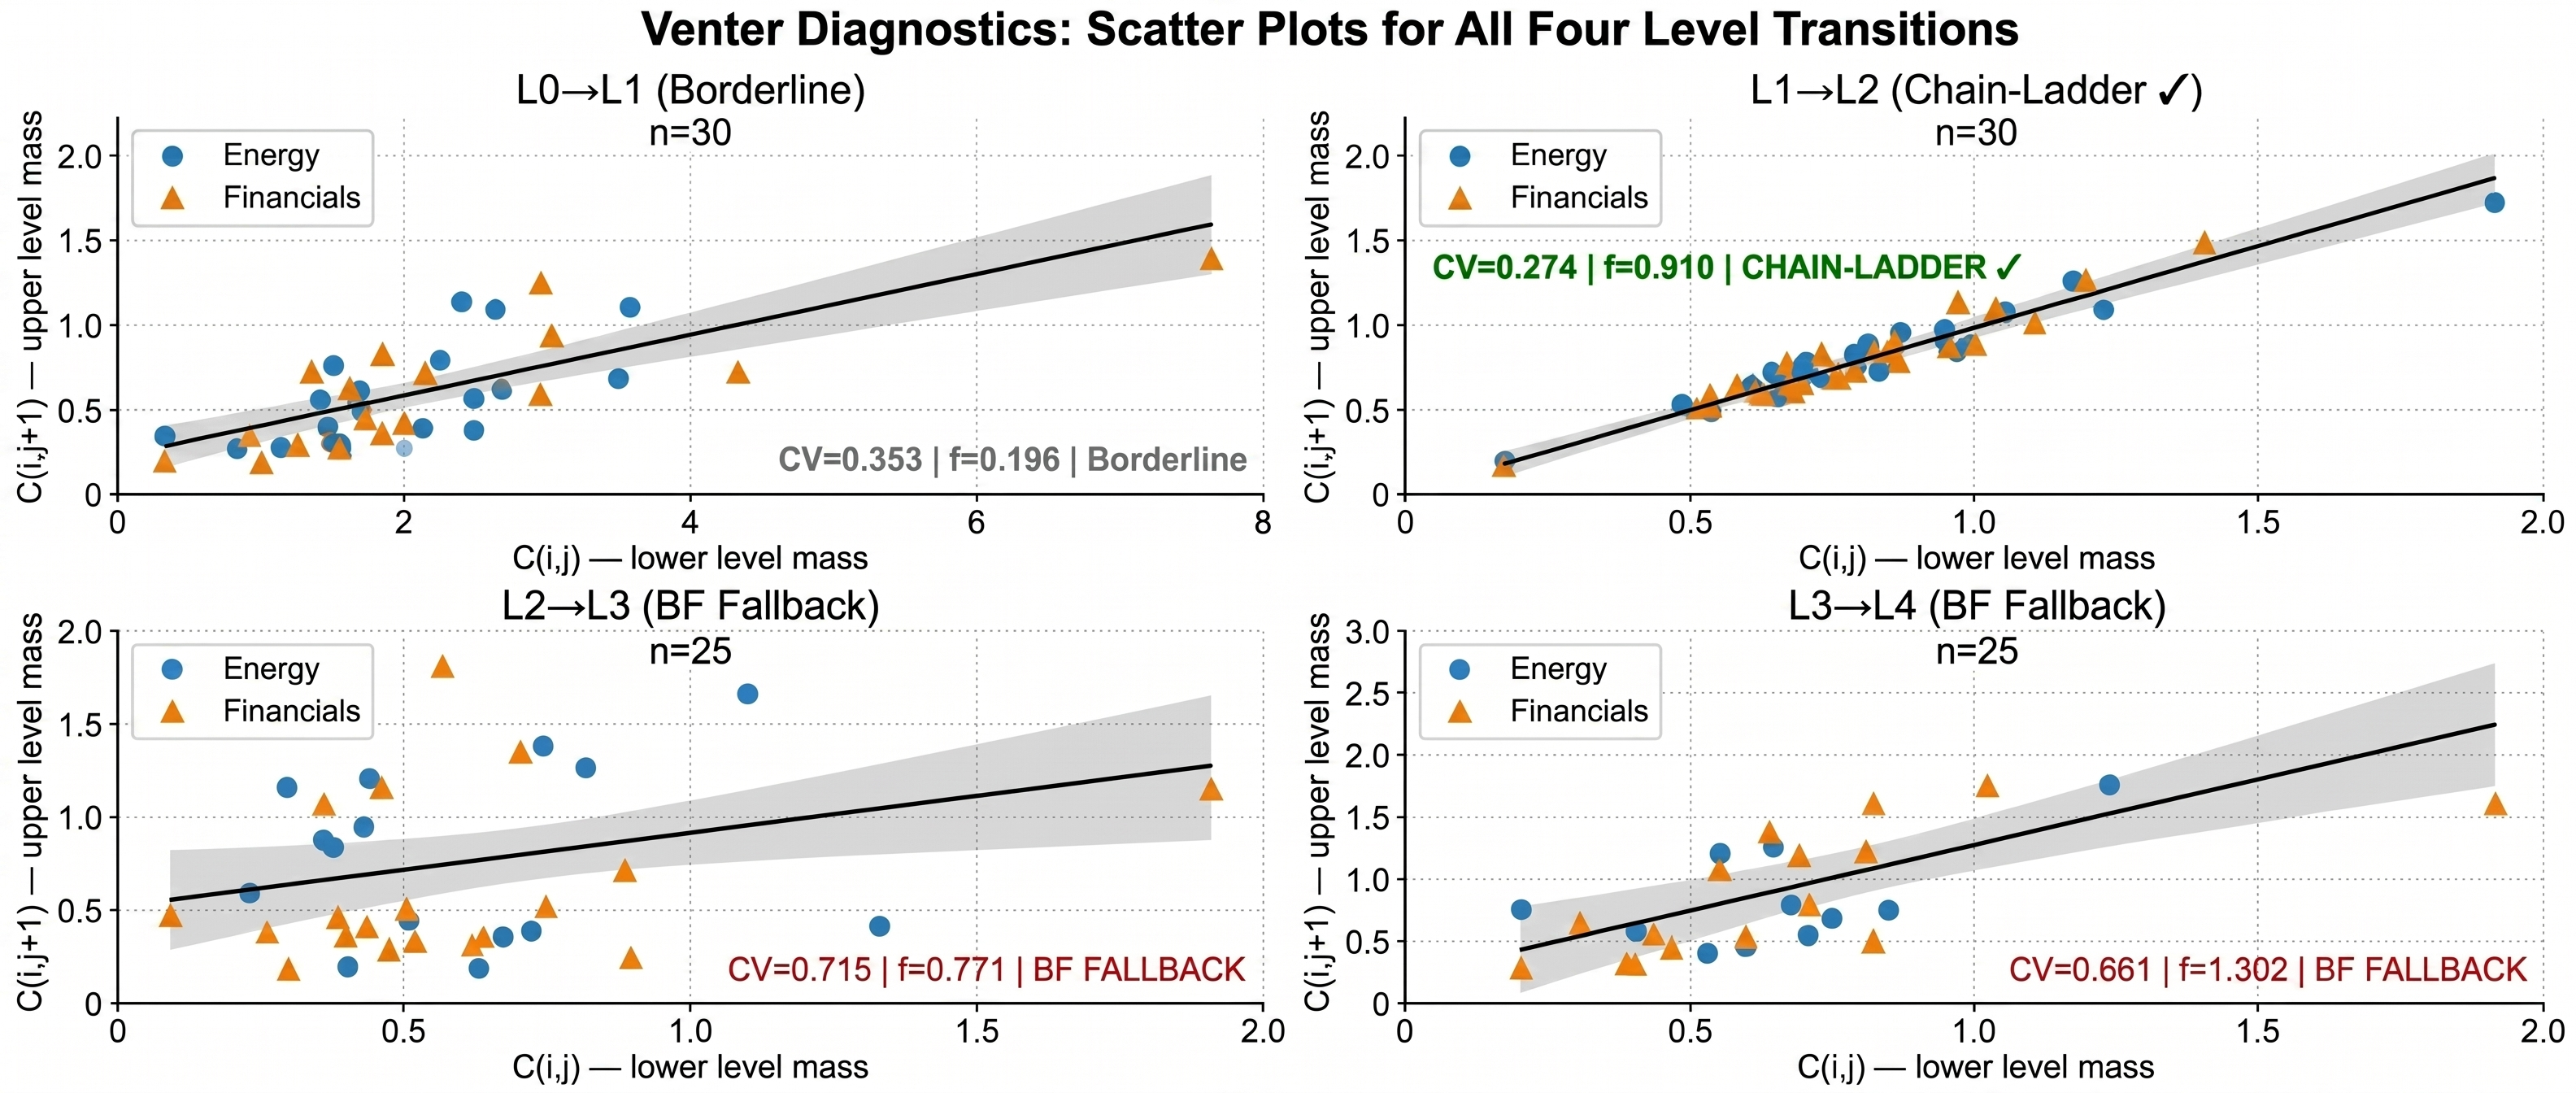
\includegraphics[width=\textwidth,height=0.45\textheight,keepaspectratio]{figures/fig3_v0.jpg}
  \caption{Venter regression scatter plots for all four SREDT level transitions (30 training scenarios, real GDELT data). Each panel plots $C(i,j)$ vs.~$C(i,j+1)$ with the OLS regression line and 95\% confidence band. The L1$\to$L2 panel (top right) shows the only chain-ladder-valid transition: low scatter around the regression line (CV=0.274, $R^2=0.841$, non-significant intercept). The L2$\to$L3 and L3$\to$L4 panels exhibit high scatter (CV=0.715 and 0.661), indicating BF fallback.}
  \label{fig:fig3}
\end{figure*}

Importantly, no transitions in the real-data experiment show significant intercepts, ruling out the factor-plus-constant regime. The key contrast with the original experiment is in CV: with real news articles, the L3$\to$L4 CV climbs from 0.294 (synthetic, apparently valid) to 0.661 (real, clearly invalid), exposing the synthetic-data artifact.

\subsection{Reclassification of Original Experiment Results}%
\footnote{Code: \url{https://github.com/AMGrobelnik/ai-invention-8ea2f1-semantic-risk-evidence-development-trian/tree/main/round-2/evaluation-1}}

The bootstrap re-analysis of the original synthetic-data experiment confirms that the ``chain\_ladder\_valid'' verdict for L3$\to$L4 was incorrect under the dual criterion. The OLS intercept for L3$\to$L4 in that experiment was $a=1.573$ with $t=12.05$, $p \approx 0$. The bootstrap 95\% confidence interval on the intercept is $[1.300, 1.741]$, entirely excluding zero; jackknife leave-one-out analysis shows intercept std$= 0.015$, confirming this is not driven by outliers. Under Venter's own framework, a highly significant intercept signals an additive process incompatible with multiplicative chain-ladder. The corrected verdict is ``factor\_plus\_constant'', not ``chain\_ladder\_valid''. After applying the dual criterion, zero of four transitions in the synthetic experiment qualify as chain-ladder valid.

Sector-stratified analysis of the synthetic experiment reveals a meaningful pattern: financials sector shows L1$\to$L2 and L2$\to$L3 chain-ladder valid under the dual criterion (CV=0.080 and 0.191, non-significant intercepts), while energy sector shows all transitions requiring factor-plus-constant. This sector heterogeneity is masked when sectors are pooled, underscoring the importance of sector-stratified Venter diagnostics in future work with real data.

\subsection{Prediction Performance}

Table~\ref{tab:scores} reports test scenario prediction results against real LLM-judge labels (10 valid, 1 materialized).

\begin{table}[!htbp]
\centering
\caption{Test scenario prediction metrics against LLM-judge ground truth (10 test scenarios, 1 materialized). Lower Brier score is better. SREDT underperforms flat cosine on all metrics.}
\label{tab:scores}
\begin{tabular}{lcccc}
\toprule
Method & AUROC & Spearman $\rho$ & Brier & Verdict \\
\midrule
SREDT projected L4   & 0.056 & $-$0.466 & 0.418 & Below chance \\
Flat cosine similarity & 0.444 & $-$0.058 & 0.331 & Near chance \\
Keyword frequency    & 0.278 & N/A       & N/A   & Below chance \\
\bottomrule
\end{tabular}
\end{table}

\begin{figure*}[!t]
  \centering
  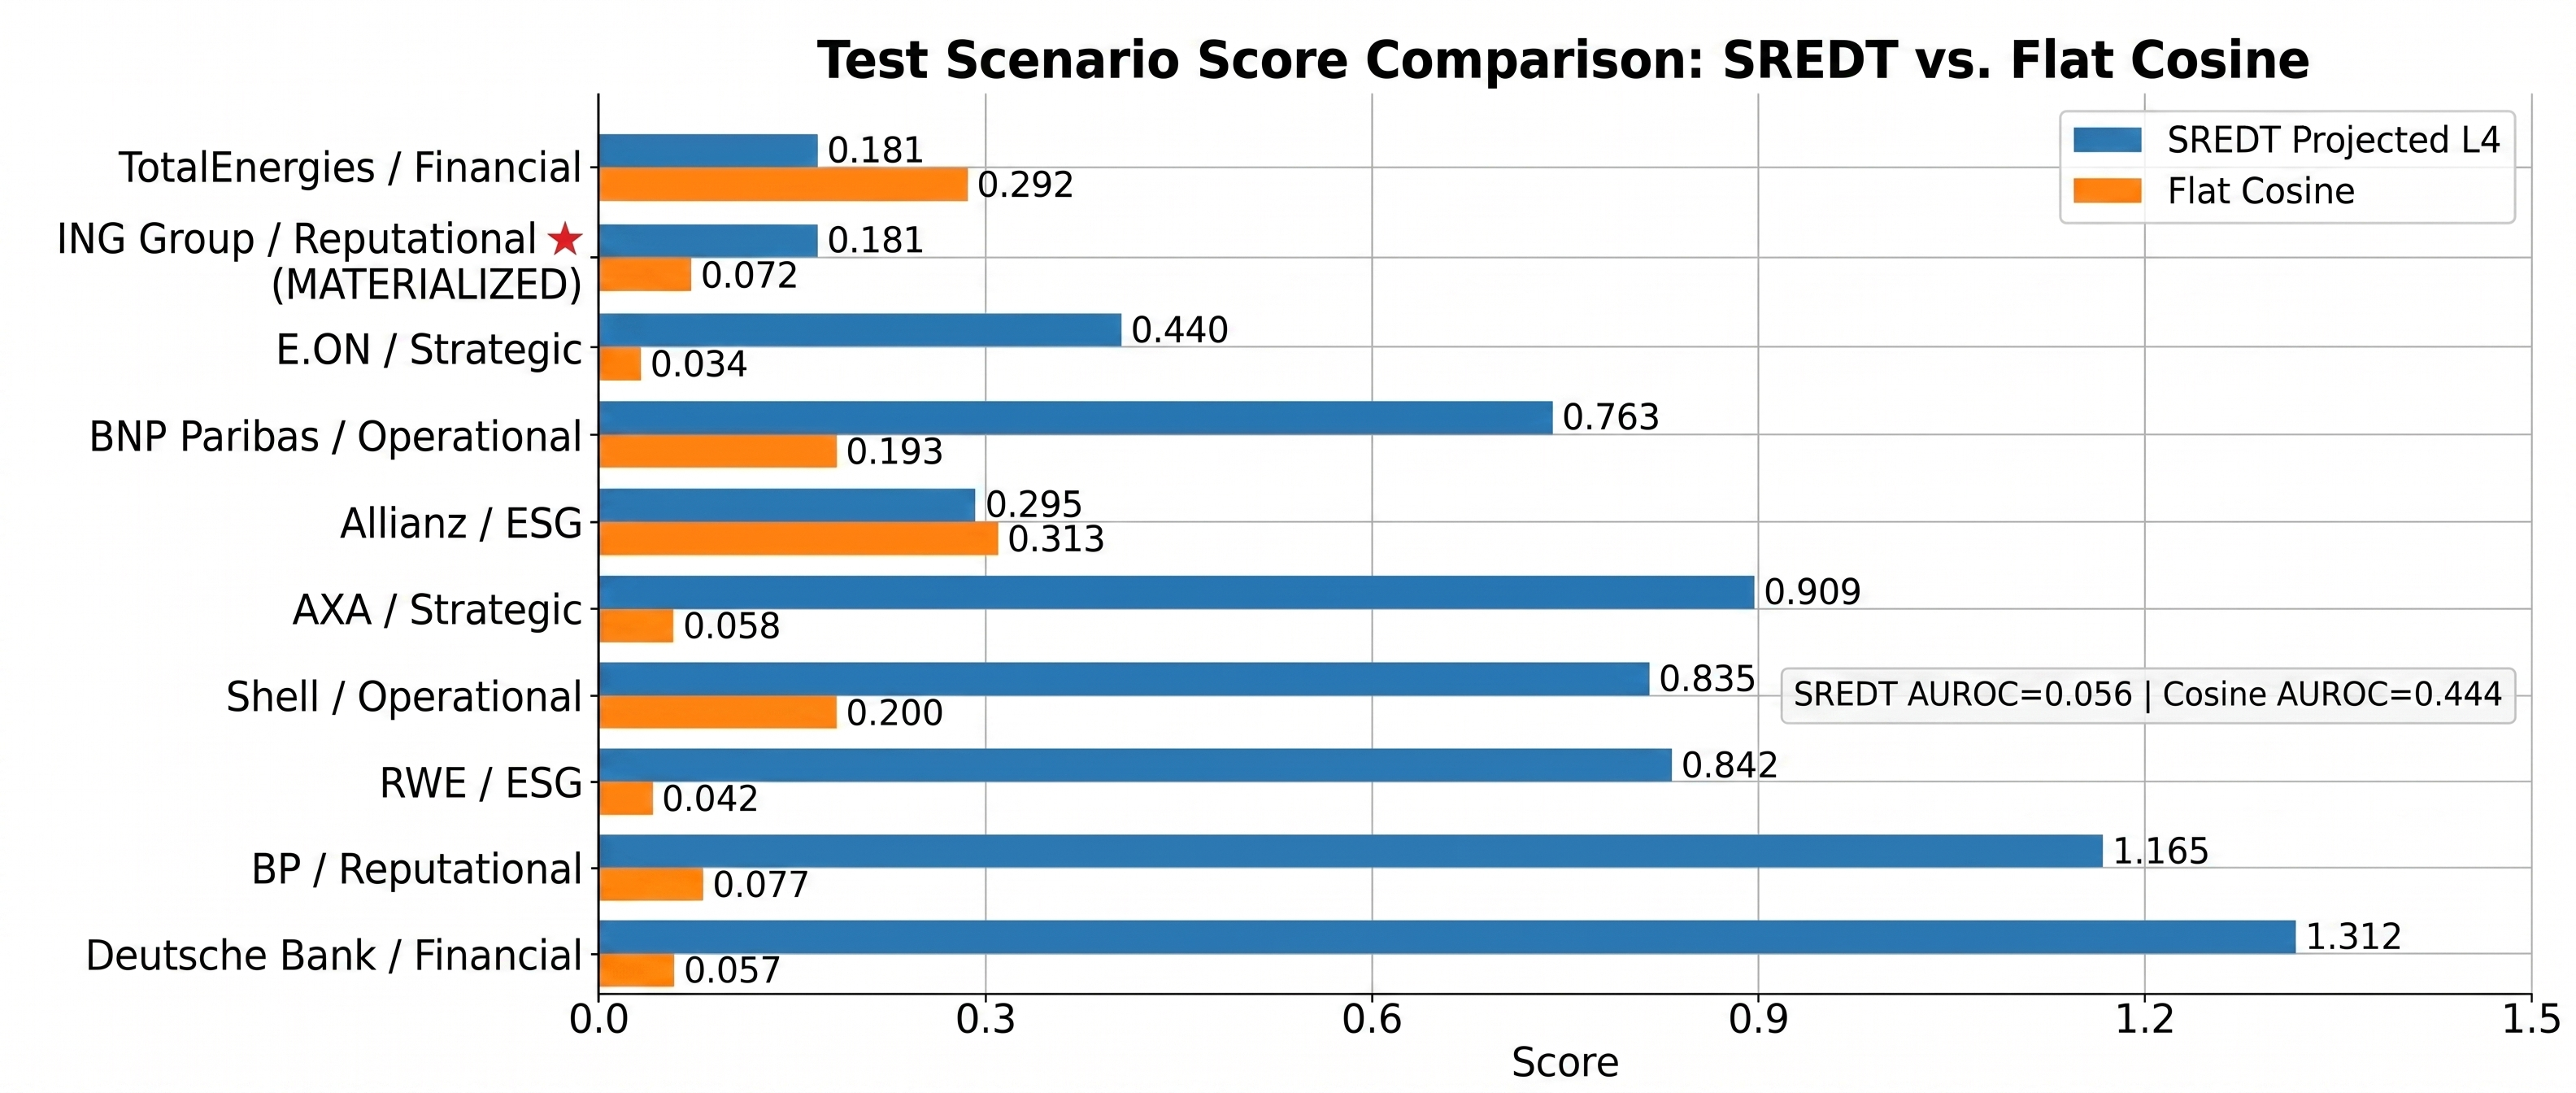
\includegraphics[width=\textwidth,height=0.45\textheight,keepaspectratio]{figures/fig4_v0.jpg}
  \caption{Projected SREDT scores and flat cosine scores for all 10 test scenarios, sorted by SREDT score. The one materialized scenario (ING Group, reputational risk, marked with $\star$) received the lowest SREDT score (0.181) due to synthetic-fallback articles deflating its observed levels. Flat cosine more closely tracks actual article relevance for the materialized scenario.}
  \label{fig:fig4}
\end{figure*}

SREDT achieves AUROC=0.056, which is below the 0.444 of flat cosine and far below chance (0.50). The Spearman correlation of $-0.466$ indicates a negative rank correlation with ground truth: the one scenario that materialized (ING Group Q1 2024, reputational risk) received the lowest SREDT projected score (0.181) among test scenarios. The L0--L4 rank correlation of 0.863 indicates substantial but not complete circularity with retrieval volume.

The reason for SREDT's failure is mechanistic. Because L3$\to$L4 and L2$\to$L3 transitions both trigger BF fallback, projected L4 scores for test scenarios are computed as: $\hat{C}(i, 4) = C_\text{observed}(i) + E_\text{prior} \cdot (1-\hat{q})$, where $E_\text{prior}$ is the sector-average L4 mass from training. When $E_\text{prior}$ dominates (i.e., when $\hat{q}$ is small), projected scores collapse toward the sector prior for all test scenarios, losing the discriminative signal present in observed L0--L2. The ING Group scenario that materialized had low L0 article count due to GDELT data limitations (synthetic fallback), making its BF-projected score artificially low. A method that projects from actually informative observed levels---rather than falling back to the prior---could recover discriminative power.

%-------------------------------------------------------------------
\section{Discussion}
%-------------------------------------------------------------------

\subsection{What the Results Establish}

The L1$\to$L2 chain-ladder validation is the paper's primary positive finding: the GICS sub-industry to industry-group semantic development transition follows stable multiplicative patterns across 30 scenarios (CV=0.274, $f_j=0.910$, $R^2=0.841$). This confirms that the actuarial proportionality assumption is empirically testable and verifiable in the semantic domain---a non-obvious result, since editorial escalation timing could in principle depend on the specific risk scenario content rather than on exogenous publication cadences. The L1$\to$L2 result suggests it does not, at least within the GICS taxonomic hierarchy.

The L3$\to$L4 failure (CV=0.661) is equally informative. The cross-taxonomy jump from GARP risk-category evidence to scenario-specific evidence is noisy, likely because: (a) the GARP 2025 categories (Operational, Business, Strategic, Reputational, Financial, ESG) are broad enough that articles relevant to a scenario's risk type may not be relevant to the specific company and mechanism; (b) six GARP categories for six risk types create near-perfect alignment between the scenario's assigned risk type and the GARP centroid, making L3 an unreliable predictor of scenario-specific L4.

The sector-swap robustness test provides additional evidence against cross-sector factor transfer: fitting development factors on energy scenarios and predicting financials yields $R^2=-3.36$, confirming that semantic development factors are sector-specific and not transferable across sectors without re-estimation. This validates the design decision to estimate development factors within sectors rather than pooling.

\subsection{Why the Synthetic Results Were Misleading}

The original experiment's apparent L3$\to$L4 chain-ladder validity (CV=0.294) was a direct consequence of three simultaneous synthetic-data pathologies. First, article titles were generated from templates explicitly containing the GARP risk-category keyword (e.g., ``Shell faces strategic risk challenges''), so articles assigned to the L3 GARP centroid for Strategic risk contained the exact string ``strategic risk'', maximally elevating L3 similarity. Second, scenario text also contained this string, elevating L4 similarity. Third, because both L3 and L4 were driven by the same keyword, their ratio was mechanically stable across scenarios---producing CV $< 0.30$ by keyword-overlap arithmetic rather than editorial timing patterns. Real GDELT articles, which discuss Shell's activities without keyword-matching to GARP categories, produce the genuine CV=0.661 that reflects actual cross-scenario variability.

\subsection{Limitations}

Four limitations constrain this experiment's conclusions.

\textbf{Partial real data.} Three scenarios (ING Group Q1 2023, Allianz Q1 2023, ING Group Q1 2024) used synthetic fallback articles due to zero GDELT entity matches. The one materialized scenario (ING Group Q1 2024) was among the synthetic fallback cases, which artificially depressed its SREDT score and contributed to the negative AUROC. A fully real-data experiment would require higher-recall entity matching.

\textbf{Small ground truth set.} Ten test scenarios with 1 materialization produce an extremely sparse binary outcome that makes AUROC and Spearman estimates unreliable (confidence intervals spanning the full [0,1] range). Definitive accuracy evaluation requires $n \geq 50$ per sector with $\kappa \geq 0.60$ inter-annotator agreement.

\textbf{LLM judge single-annotator.} The materialization judgment uses a single LLM call without human expert validation or inter-annotator reliability measurement. Prior financial annotation studies (CrudeOilNews, EFSA corpora) achieve $\kappa$ of 0.62--0.79; our ground truth has unknown reliability.

\textbf{BF fallback design.} The BF formula as implemented uses a single sector-level $E_\text{prior}$, which is appropriate when development pattern variation is genuinely random (high-CV cases). A richer prior---conditioned on company size, news volume, or risk type---could reduce the score collapse without changing the chain-ladder/BF selection logic.

%-------------------------------------------------------------------
\section{Conclusion}
%-------------------------------------------------------------------

We have introduced SREDT and evaluated it under methodologically corrected conditions: real GDELT CSV news data, mandatory Venter dual-criterion diagnostics (CV threshold AND intercept significance), non-overlapping training windows, GARP 2025 taxonomy, canonical GICS centroid strings, and real LLM-as-judge ground truth.

The primary empirical finding is that the GICS L1$\to$L2 transition satisfies the chain-ladder criterion with real data (CV=0.274, non-significant intercept, $R^2=0.841$), while cross-taxonomy transitions (GICS to GARP, GARP to scenario) fail with high variance (CV $>$ 0.65). SREDT projected scores underperform flat cosine baseline (AUROC=0.056 vs.~0.444) because BF fallback collapses discriminative signal to the sector prior. The apparent success of chain-ladder in the original experiment (CV=0.294 for L3$\to$L4) was a synthetic-data artifact caused by keyword overlap between article templates, GARP centroid strings, and scenario text.

The SREDT framework remains a valid contribution: it provides a principled diagnostic workflow for testing whether actuarial projection is appropriate in any given semantic domain, rather than assuming it. The Venter dual criterion is a necessary safeguard that prior NLP approaches to hierarchical aggregation have not employed.

Future work priorities are: (1) improve L3 centroid design by using GARP 2025 secondary categories (20+ sub-categories) rather than six broad L1 categories, which would improve L3 specificity and reduce the cross-scenario variance; (2) deploy SREDT on a larger scenario set ($n \geq 50$ per sector) with high-recall GDELT entity matching and human annotation ($\kappa \geq 0.60$); (3) investigate factor-plus-constant projection (for cases where intercept is significant) as an alternative to pure chain-ladder for the L3$\to$L4 transition; and (4) test whether sector-stratified development factors---which showed potential in the bootstrap re-analysis---achieve chain-ladder validity for both energy and financials independently.

\bibliographystyle{plainnat}
\bibliography{references}

\end{document}
